\documentclass[
  11pt,
  letterpaper,
   addpoints,
   %answers
  ]{exam}

\usepackage{../exercise-preamble}
\usepackage{float}
\begin{document}

\noindent
\begin{minipage}{0.47\textwidth}

\includegraphics[width=\textwidth]{../fcfm_die}
\end{minipage}
\begin{minipage}{0.53\textwidth}
\begin{center} 
\large\textbf{Conversión de la Energía y Sistemas Eléctricos} (EL4111) \\
\large\textbf{Clase particular Jelu (12-09-2025 - 21:00)} \\
\small Erik Sáez\\
\end{center}
\end{minipage}

\vspace{0.5cm}
\noindent
\vspace{.85cm}

\begin{questions}
    %---------------------------------------------------------------
    \question  Considere el circuito magnético de la Figura~\ref{fig:circuito-magnetico}, el cual se compone de dos núcleos con permeabilidad magnética $\mu_r \to \infty$ y cuya sección transversal es $s = 4\,\mathrm{mm^2}$. Los núcleos están separados por una distancia $g = 5\,\mathrm{mm}$ y $\delta = 4\,\mathrm{cm}$ como se muestra en la figura. Además, el circuito cuenta con dos enrollados con $N_1 = 300$ y $N_2 = 200$ vueltas, respectivamente, por los cuales se hace fluir una corriente de $i_1 = 20\,\mathrm{A}$ e $i_2 = 10\,\mathrm{A}$.

\begin{figure}[H]
  \centering
    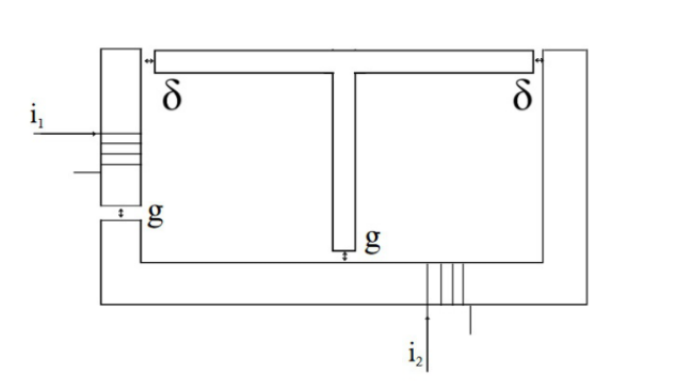
\includegraphics[width=0.6\textwidth]{Jelu_01}
  \caption{Circuito magnético con dos núcleos, enrollados $N_1$ y $N_2$, y corrientes $i_1$ e $i_2$. El entrehierro está definido por $g$ y $\delta$.}
  \label{fig:circuito-magnetico}
\end{figure}

\begin{parts}
  \part Calcular las reluctancias del sistema.
  \part Dibujar el circuito magnético equivalente.
  \part Calcular las inductancias propias y mutuas del circuito.
  \part Calcular la energía total acumulada.
  \part Calcular la energía total acumulada para el caso ideal donde $g=\delta=0$.
\end{parts}
%---------------------------------------------------------------
\begin{solution}

\subsection*{Resolución 1.1}
Buscamos el obtener las reluctanica del sistema, por lo tanto en relacion a los datos entregado del enunciado tenemos que: 
\begin{align}
R_g &= \frac{g}{\mu_0 A}
     = \frac{5\cdot10^{-3}}{(4\pi\cdot10^{-7})(4\cdot10^{-6})}
     = 9.9472\times10^{8}\;[\text{A/Wb}], \\
R_\delta &= \frac{\delta}{\mu_0 A}
     = \frac{4\cdot10^{-2}}{(4\pi\cdot10^{-7})(4\cdot10^{-6})}
     = 7.9577\times10^{9}\;[\text{A/Wb}].
\end{align}
Con lo que se obtienen las reluctancias del sistema.
\subsection*{Resolución 1.2}
Se busca obtener el circuito magnetico equivalente, que de manera rapida se tiene que debido a las reluctancias y las bobinas. El circuito equivalente es:
\begin{figure}[H]
  \centering
  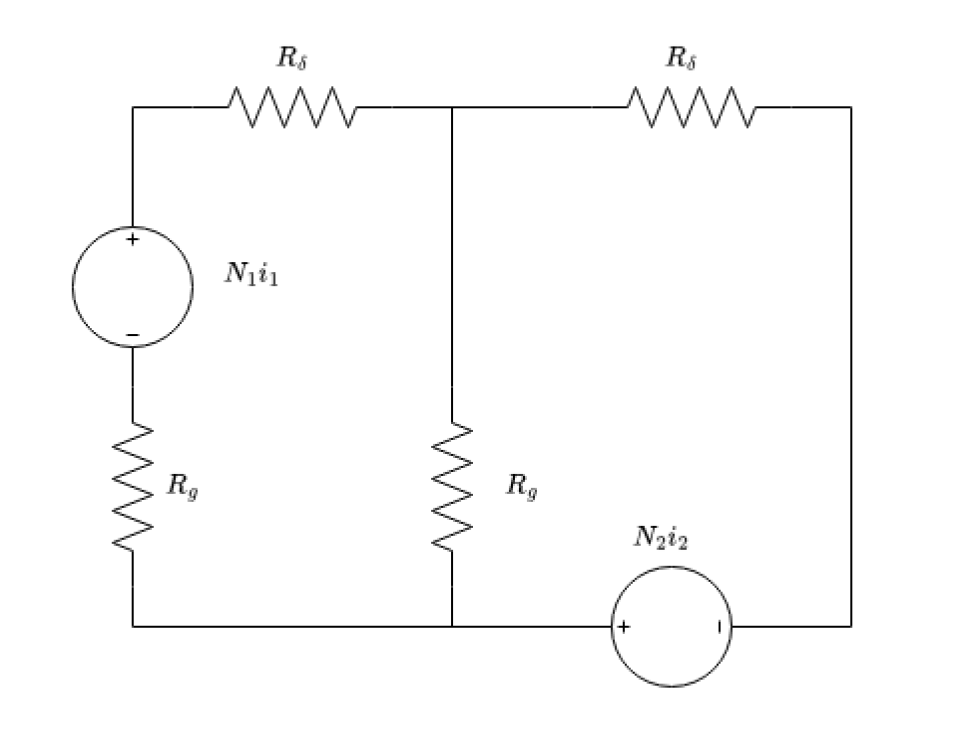
\includegraphics[width=0.5\linewidth]{Jelu_02}
  \caption{Circuito magnético equivalente.}
\end{figure}

\subsection*{Resolución 1.3}
Luego se busca el calcular las inductancias propias y mutuas del circuito por lo que para calcular $L_11$ Cortocircuitando la segunda fuente (bobina 2):
\begin{figure}[H]
  \centering
  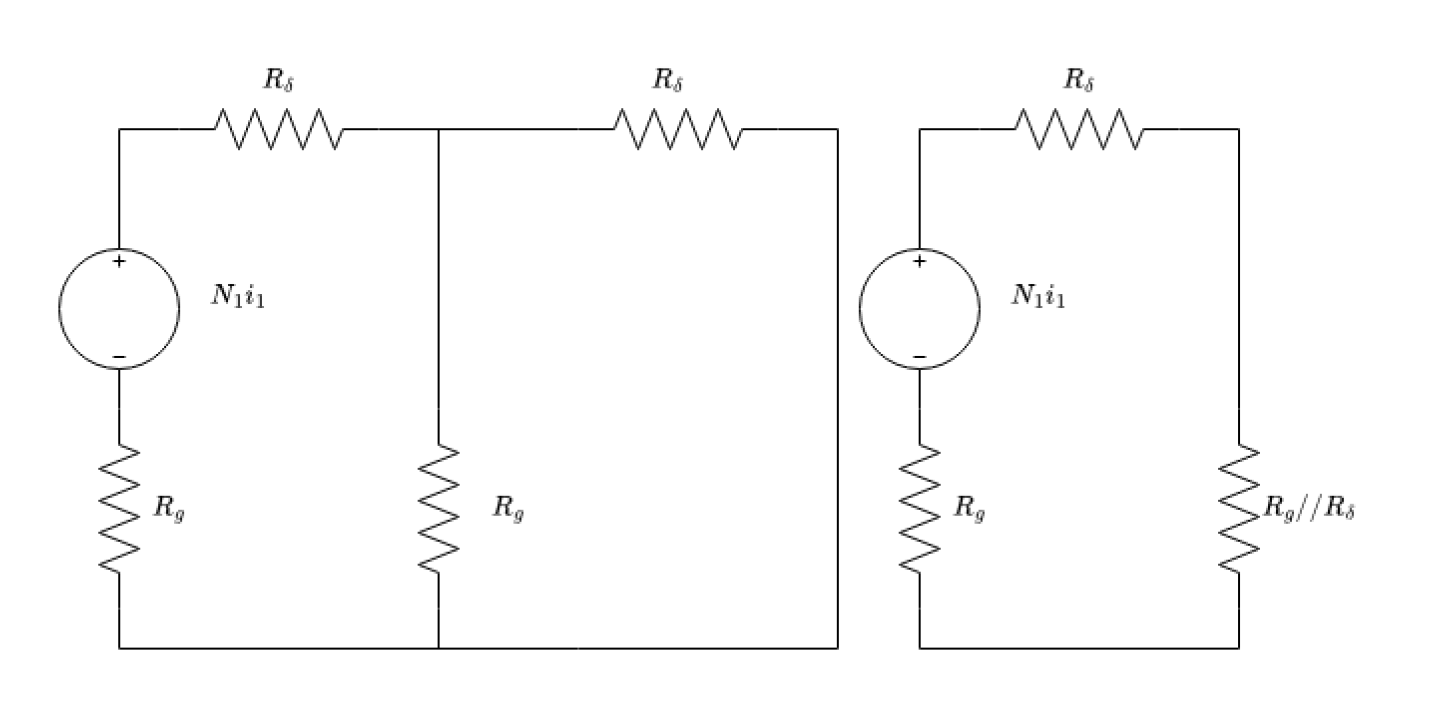
\includegraphics[width=.6\linewidth]{Jelu_03}
  \caption{Esquema usado para calcular \(L_{11}\).}
\end{figure}
\begin{align}
R_{\text{eq}} &= (R_g \parallel R_\delta) + R_g + R_\delta
               = 9.8367\times 10^{9}\;[\text{A/Wb}],\\
N_1 i_1 &= \phi_{11} R_{\text{eq}}, \qquad
\phi_{11}=\frac{N_1 i_1}{R_{\text{eq}}}, \\
L_{11} &= \frac{N_1\phi_{11}}{i_1}=\frac{N_1^2}{R_{\text{eq}}}
       = 9.1494\times10^{-6}\;[\text{H}].
\end{align}
De forma analoga tenemos que para calcular \(L_{22}\) cortocircuitando la primera fuente (bobina 1):
\begin{figure}[H]
  \centering
  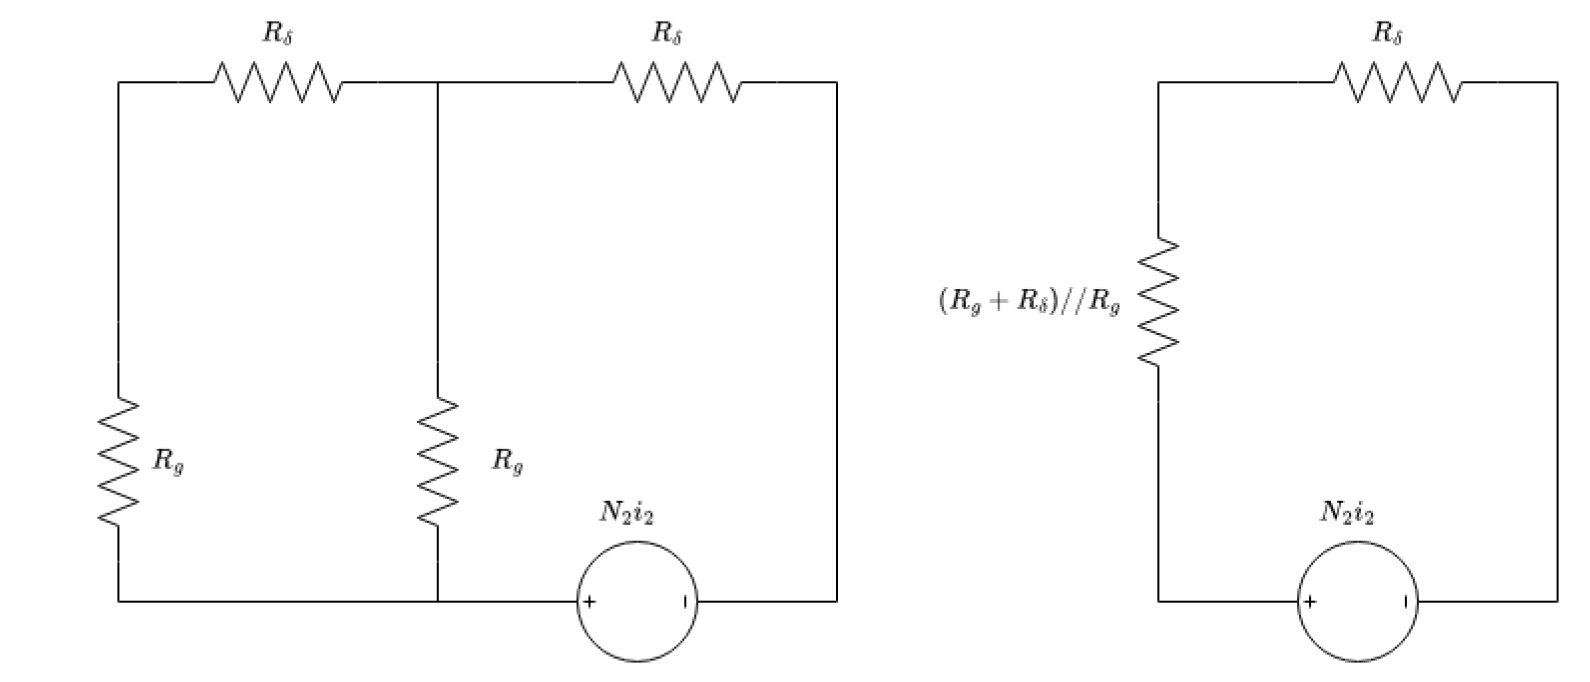
\includegraphics[width=.6\linewidth]{Jelu_04}
  \caption{Esquema usado para calcular \(L_{22}\).}
\end{figure}
En donde tenemos que :
\begin{align}
R_{\text{eq}} &= (R_g + R_\delta) \parallel (R_g) + R_\delta
               = 8.853 \cdot 10^{9}\;[\text{A/Wb}],\\
N_2 i_2 &= \phi_{22} R_{\text{eq}}, \qquad
\phi_{22}=\frac{N_2 i_2}{R_{\text{eq}}}, \\
L_{22} &= \frac{N_2\phi_{22}}{i_2}=\frac{N_2^2}{R_{\text{eq}}}
       = 4.5183\times10^{-6}\;[\text{H}].
\end{align}
Finalmente para calcular \(L_{12}\) se tiene el siguiente circuito:
\begin{figure}[H]
    \centering
    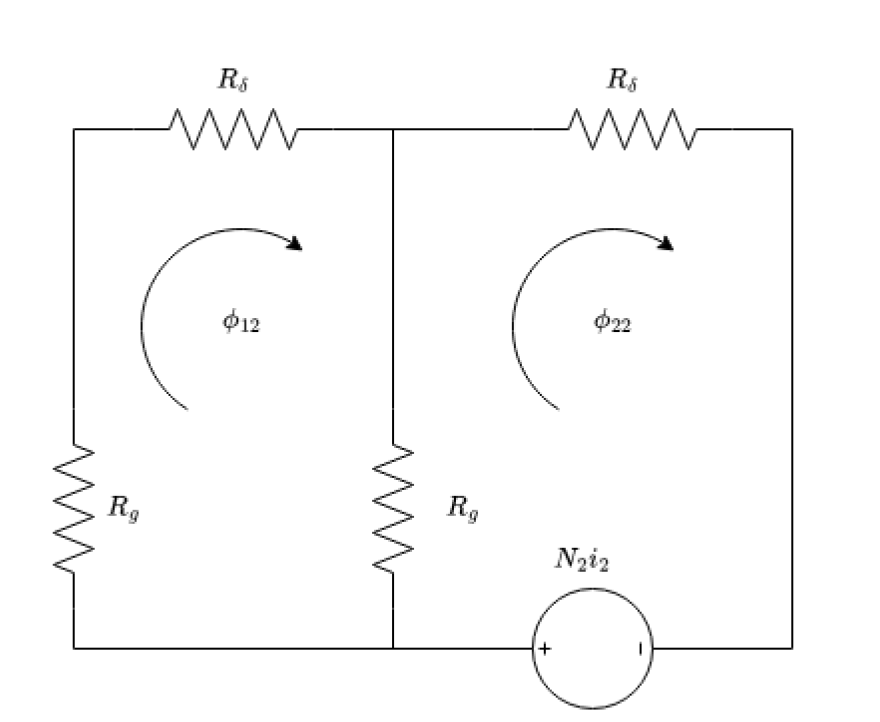
\includegraphics[width=.6\linewidth]{Jelu_05}
    \caption{Esquema usado para calcular \(L_{12}\).}
\end{figure}
De la malla de $\phi_{12}$ se tiene:
\begin{align}
    \phi_{12} R_\delta + \phi_{12} R_g + R_g (\phi_{12} - \phi_{22}) &= 0 \\
    2\phi_{12} R_\delta + \phi_{12} R_g &= \phi_{22} R_g \\
    \phi_{12}(2R_\delta + R_g) &= \phi_{22} R_g \\
    \phi_{12} &= \frac{R_g \phi_{22}}{R_\delta + 2R_g}
\end{align}

Donde $\phi_{22}$ es el obtenido al calcular $L_{22}$. Luego:
\begin{align}
    L_{12} &= \frac{N_1}{i_2} \phi_{12} = \frac{N_1}{i_2} \cdot \frac{R_g}{2R_\delta + R_g} \cdot \frac{N_2 i_2}{R_{eq}} \\
    L_{12} &= \frac{N_1 N_2 R_g}{R_{eq}(R_\delta + 2R_g)} = 6.7773 \cdot 10^{-7}~[H]
\end{align}
Para $L_21$ el procedimiento es bastante similar, tenemos el siguiente circuito dado por:
\begin{figure}[H]
    \centering
    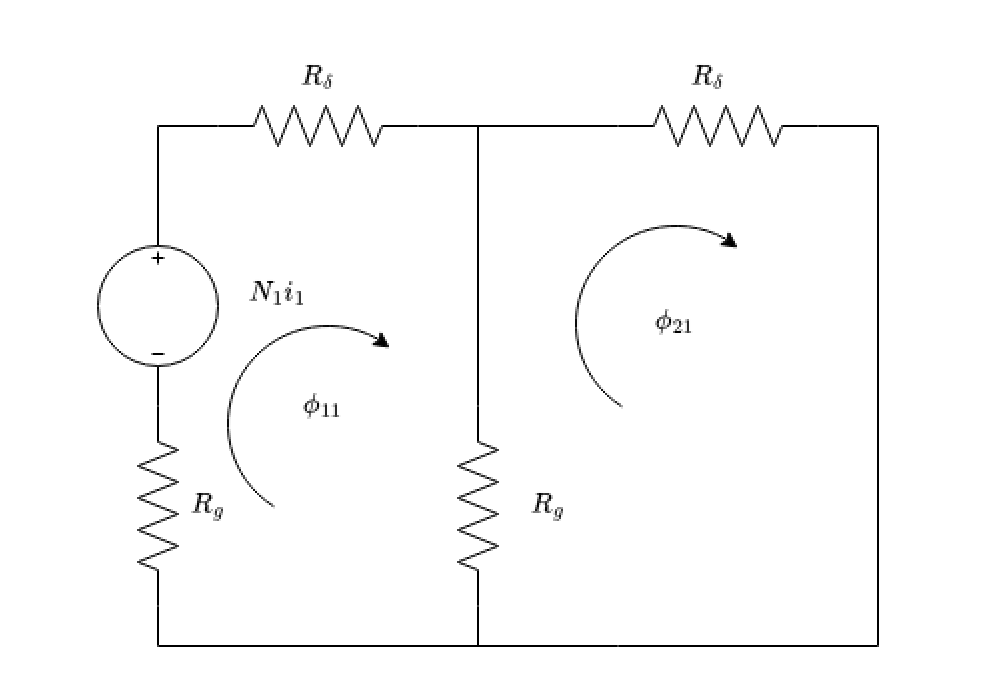
\includegraphics[width=.6\linewidth]{Jelu_06}
    \caption{Esquema usado para calcular \(L_{21}\).}
\end{figure}
De donde se tiene la malla:
\begin{align}
    \phi_{21} R_\delta + R_g (\phi_{21} - \phi_{11}) &= 0 \\
    \phi_{21} &= \frac{R_g}{R_\delta + R_g} \phi_{11}
\end{align}

Finalmente, utilizando el flujo $\phi_{11}$ y $R_{eq}$ obtenidos al calcular $L_{11}$:
\begin{align}
    L_{21} &= \frac{N_2 \phi_{21}}{i_1} = \frac{N_2 N_1 R_g}{R_{eq}(R_\delta + R_g)} \\
    L_{21} &= 6.7774 \cdot 10^{-7}~[H]
\end{align}
\subsection*{Resolución 1.4}
Luego usando las inductancias calculadas en la parte anterior, tenemos que la energia se calcula como:
\begin{align}
    W= \frac{1}{2}\left(L_{11}i_1^2 + L_{22}i_2^2 + (L_{12}+L_{21})i_1 i_2\right)
    = 2.1913\times10^{-3}\;[\text{J}].
\end{align}
Con lo que se obtiene la energia total acumulada en el sistema.
\subsection*{Resolución 1.5}
Buscamos analizar la energia acumulada en el caso ideal donde $g=\delta=0$, por lo que en este caso las reluctancias seran nulas, es decir, Luego
\begin{align}
  L \propto \frac{1}{R} \to \infty
\end{align}
Por lo que las inductancias seran infinitas, y por lo tanto la energia acumulada tambien sera infinita.
\end{solution}
%---------------------------------------------------------------
\newpage
\question Considere dos transformadores ideales, con las siguientes características:
\begin{itemize}
  \item \textbf{Transformador 1}: relación de vueltas \(N_1/N_2 = 3:1\), polaridad sustractiva.
  \item \textbf{Transformador 2}: relación de vueltas \(N_1/N_2 = 1:2\), polaridad aditiva.
\end{itemize}

Estos transformadores alimentan tres cargas:
\(Z_1 = 5 + j2\,[\Omega]\), \(Z_2 = 25 + j12\,[\Omega]\) y \(Z_3 = 10 + j5\,[\Omega]\),
conectadas como se muestra en la Figura~\ref{fig:trafos}. Además, se conecta una
fuente \(V\) al Transformador 1 como se indica en la figura.

\begin{figure}[H]
  \centering
    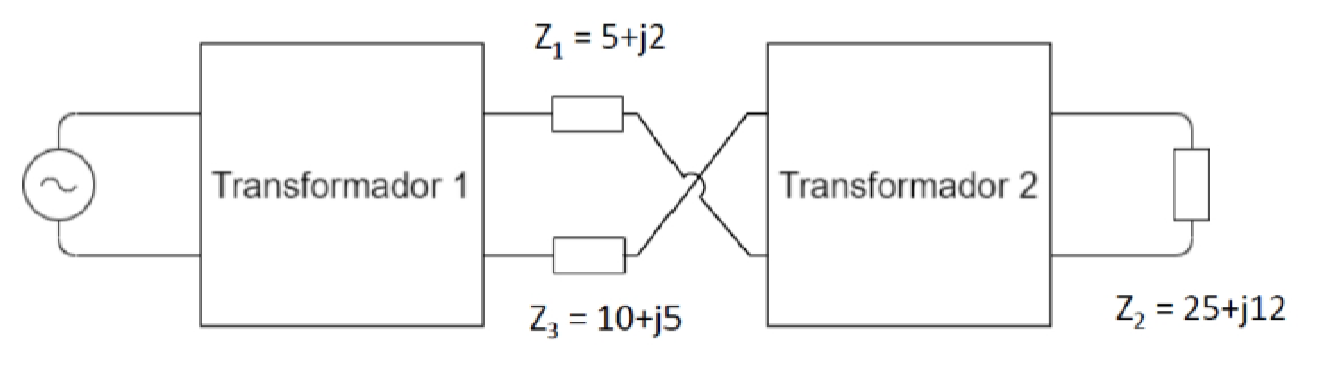
\includegraphics[width=0.7\textwidth]{Jelu_07}
    \caption{Banco de transformadores y cargas: esquema general del sistema trifásico con transformadores y conexiones de carga.}
    % alt: Esquema de transformadores y cargas mostrando conexiones primarias y secundarias.
  \label{fig:trafos}
\end{figure}

\begin{parts}
  \part Plantee las ecuaciones eléctricas y magnéticas involucradas.
  \part Calcule las corrientes en el primario y secundario de ambos transformadores
        si el primario del Transformador 1 se alimenta con una fuente de tensión
        \(V = 220\angle 0^{\circ}\,[\text{V}]\).
  \part Calcule la caída de tensión en cada carga y las potencias \(P\) y \(Q\) de las mismas.
\end{parts}
%---------------------------------------------------------------
\begin{solution}

\subsection*{Resolución 2.1}
Lo primero es plantear las ecuaciones eléctricas y magnéticas involucradas, para
lo cual recordamos que para transformadores ideales, se cumple que:
\begin{align}
\frac{V_1}{V_2}=\frac{N_1}{N_2},\qquad
\frac{i_1}{i_2}=\frac{N_2}{N_1},\qquad
Z_1 = Z_2\left(\frac{N_1}{N_2}\right)^{\!2},\qquad
S_1=S_2.
\end{align}
Donde tenemos los siguientes datos de utilidad:
\begin{align}
\text{T1: } \frac{N_1}{N_2}=3{:}1\ (\text{sustractiva}),\qquad
\text{T2: } \frac{N_1}{N_2}=1{:}2\ (\text{aditiva}),
\quad Z_1=5+j2,\; Z_2=25+j12,\; Z_3=10+j5.
\end{align}
\begin{figure}[H]
  \centering
  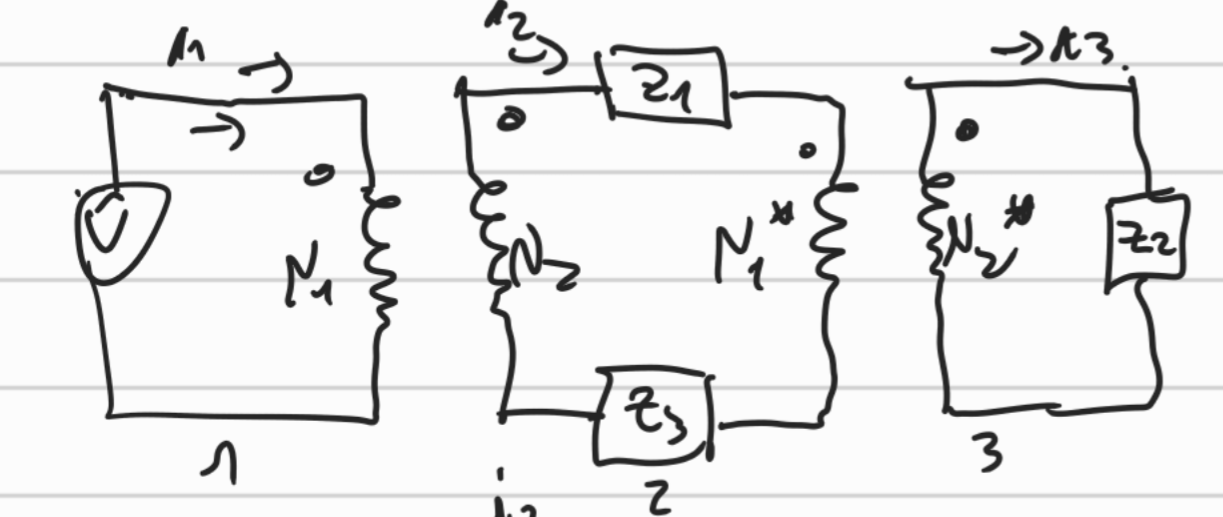
\includegraphics[width=0.6\linewidth]{Jelu_08}
  \caption{Fasores y triángulo de tensiones de línea: representación polar de $V_{AB},V_{BC},V_{CA}$ y fasores de fase.}
  % alt: Círculo con triángulo equilátero que muestra tensiones de línea (verde) y fasores de fase (azul) con V_{AN} en rojo.
\end{figure}

\subsection*{Resolución 2.2}
Luego debemos calcular las corrientes en primario y secundarios, para lo cual primero referimos, es decir:
\begin{align}
    Z_2''&= Z_2\left(\frac{N_1^*}{N_2^*}\right)^{\!2} \\
Z_2''&=(25+j12)\Big(\tfrac{1}{2}\Big)^2=6.25+j3~[\Omega].
\end{align}
Luego podemos calcular la impedancia equivalente viene dada por:
\begin{align}
    Z_{eq}'' &= Z_{1} + Z_2'' + Z_3 \\
    &= (5+j2) + (6.25+j3) + (10+j5) = 21.25 + j10~[\Omega]
\end{align}
\begin{figure}[H]
  \centering
  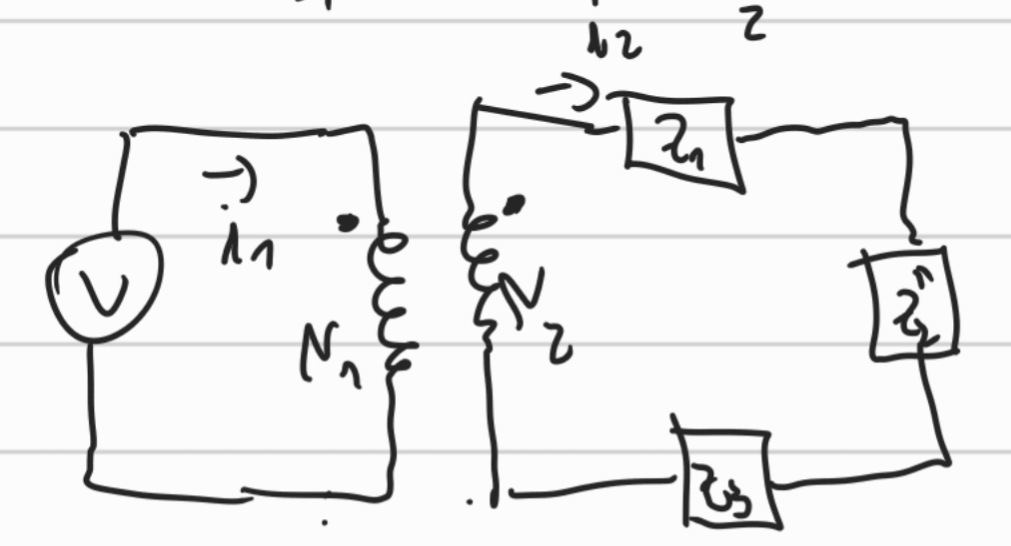
\includegraphics[width=0.5\linewidth]{Jelu_09}
  \caption{Convención de referencia de fases: A = 0° y orientación de tensiones de línea en secuencia positiva.}
  % alt: Triángulo con vértices A(0°), B(120°), C(240°) y el fasor $V_{AN}$ apuntando al neutro N.
\end{figure}
Luego tenemos que volver a referir, por lo que tendremos que:
\begin{align}
    Z_{eq}' &= Z_{eq}'' \left(\frac{N_1}{N_2}\right)^2 \\
    &= (21.25 + j10) \cdot \left(\frac{3}{1}\right)^2\\
    &= 191.25 + j90~[\Omega].
\end{align}
Con lo que finalmente podemos obtener la corriente en el primario del Transformador 1, es decir:
\begin{align}
    V&= i_1 \cdot Z_{eq}' \\
    i_1 &= \frac{V}{Z_{eq}'}\\
    &= \frac{220\angle0^\circ}{191.25 + j90} = 1.0408\angle(-25.2^\circ)\;[\mathrm{A}].
\end{align}
\begin{figure}[H]
  \centering
  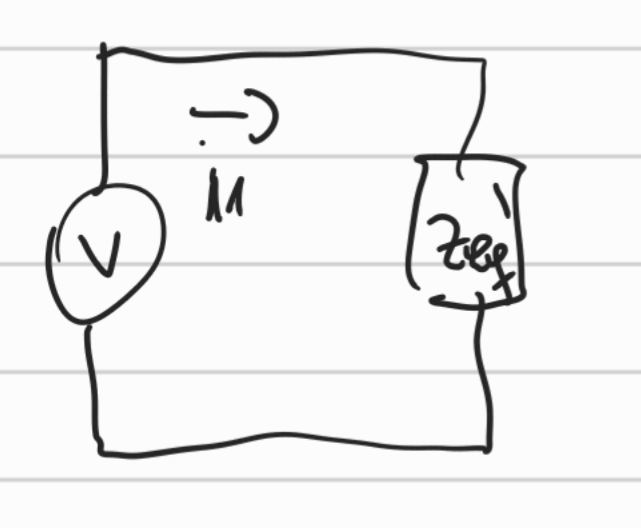
\includegraphics[width=0.3\linewidth]{Jelu_10}
  \caption{Fasores de fase referidos al neutro $N$: $V_{AN}$, $V_{BN}$ y $V_{CN}$ en un sistema balanceado.}
  % alt: Tres fasores simétricos desde el neutro hacia A,B,C en 0°,120° y 240° que representan tensiones de fase.
\end{figure}
Luego volvemos a referenciar para obtener las corrientes de los demas transformadores como:
\begin{align}
    \frac{i_1}{i_2} &= \frac{N_2}{N_1} \\
    i_2 &= \frac{N_1}{N_2} i_1\\
    &= 3 \cdot 1.0408\angle(-25.2^\circ) = 3.1225\angle(-25.2^\circ)\;[\mathrm{A}], \\
\end{align}
Luego tenemos que para el otro transformado se cumple que:
\begin{align}
    \frac{i_2}{i_3} &= \frac{N_2^*}{N_1^*} \\
    i_3 &= \frac{N_1^*}{N_2^*} i_2\\
    &= \frac{1}{2} \cdot 3.1225\angle(-25.2^\circ) = 1.5613\angle(-25.2^\circ)\;[\mathrm{A}].
\end{align}
Con lo que se obtiene todo lo solicitado en esta parte.
\subsection*{Resolucion 2.3}
Se busca obtener la caida de tension en cada carga y las potencias P y Q por lo cual tenemos que:
\begin{align}
    V_{Z_1}&=i_2 Z_1=16.8752\angle(-3.39^\circ)\ \mathrm{V},\\
    V_{Z_2}&=i_3 Z_2=43.2949\angle(0.44^\circ)\ \mathrm{V},\\
    V_{Z_3}&=i_2 Z_3=34.9103\angle(1.36^\circ)\ \mathrm{V}.
\end{align}
Luego podemos calcular tanto el P y Q recordando que:
\begin{align}
    S = V \cdot i^{*} = i \cdot Z \cdot i^{*} = |i|^2 \cdot Z
\end{align}
Donde tenemos que:
\begin{align}
  Z &= R + jX, \\
  S &= P + jQ, \\
  P &= |i|^2 R = \Re\{S\}, \\
  Q &= |i|^2 X = \Im\{S\}
\end{align}
De esta manera tenemos que finalmente:
\begin{align}
    P_{Z_1}&=48.74~\mathrm{W}, &Q_{Z_1}&=19.5~\mathrm{VAr},\\
    P_{Z_2}&=60.9375~\mathrm{W}, &Q_{Z_2}&=29.25~\mathrm{VAr},\\
    P_{Z_3}&=97.5~\mathrm{W}, &Q_{Z_3}&=48.75~\mathrm{VAr}.
\end{align}
\end{solution}
\newpage
\question La figura ilustra dos transformadores trifásicos de \(250~\text{kVA}\), \(33/12~\text{kV}\), \(50~\text{Hz}\).
El grupo de conexión del primer transformador es \(\mathrm{Yd11}\), mientras que el del segundo es \(\mathrm{Dy7}\).

\begin{parts}
  \part Si se quisiera conectar ambos transformadores en paralelo, ¿qué terminales secundarios se deben conectar entre sí?
  \part Si los enrollados de AT de ambos transformadores se conectan a tensión trifásica nominal, como se indica en la figura, ¿cuál sería la lectura de los voltímetros?
\end{parts}

\begin{figure}[h!]
  \centering
    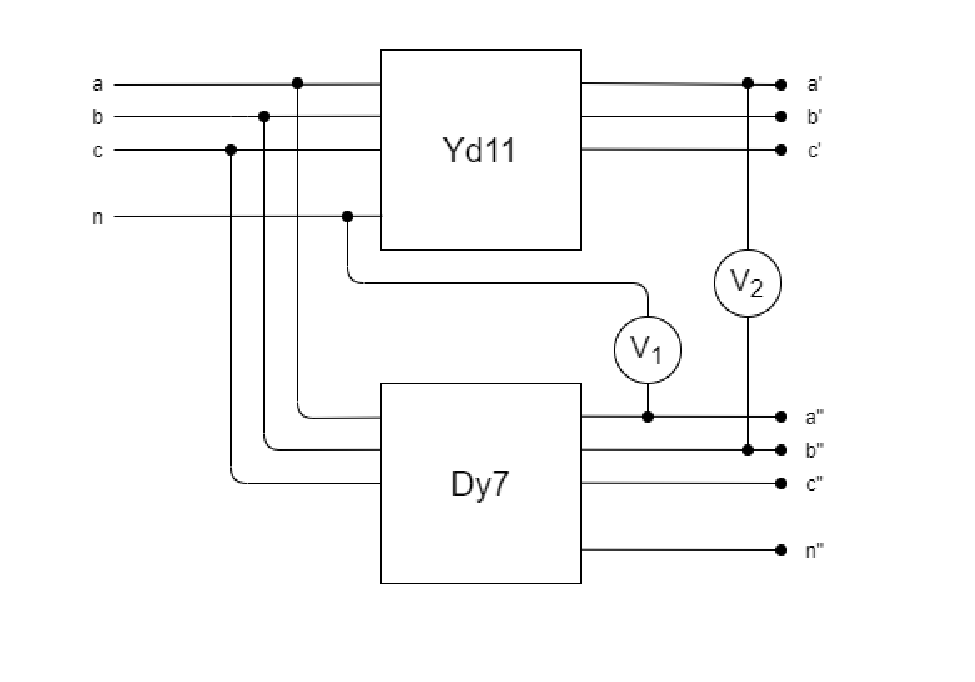
\includegraphics[width=0.6\textwidth]{Jelu_11}
  \caption{Esquema de conexión de los dos transformadores.}
  \label{fig:trafos-paralelo}
\end{figure}
%---------------------------------------------------------------
\begin{solution}

\subsection*{Resolución 3.1}
Para operación en paralelo no debe existir diferencia de tensión (ni en magnitud ni en ángulo) entre las bornas que se unan.
\begin{figure}[H]
  \centering
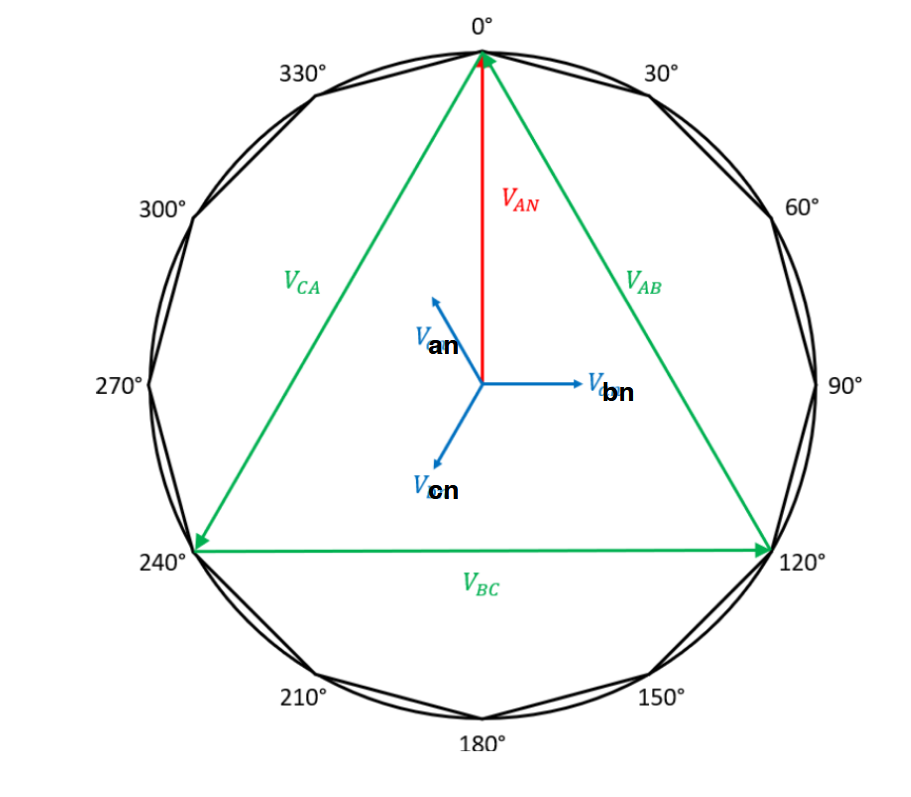
\includegraphics[width=0.6\linewidth]{Jelu_17}
  \caption{Esquema de conexiones de banco de transformadores: lado de alta tensión (AT) en \textbf{Delta} y lado de baja tensión (BT) en \textbf{Estrella} (Y). Las líneas verdes muestran la conexión en triángulo y las azules la conexión en estrella.}
  % alt: Diagrama de tres transformadores con conexiones primarias en Delta y secundarias en Estrella (Y).
\end{figure}
\begin{equation}
V_{LL}=33~\text{kV},\qquad 
V_{FN}=\frac{V_{LL}}{\sqrt{3}}=19.0526~\text{kV}.
\end{equation}

\begin{align}
\underline{V}_a&=19.0526\angle 0^\circ,
&
\underline{V}_b&=19.0526\angle (-120^\circ),
&
\underline{V}_c&=19.0526\angle 120^\circ
\quad [\text{kV}_{FN}].
\end{align}

Relación de tensiones (ideal) \(k=\tfrac{N_2}{N_1}=\tfrac{12}{33}\).

\textbf{T1 (Yd11, desfase \(11\times30^\circ=330^\circ\))}:
\begin{align}
\underline{V}_{a'}&=k\,\underline{V}_a\angle(-330^\circ)=6.9288\angle 30^\circ,\\
\underline{V}_{b'}&=k\,\underline{V}_b\angle(-330^\circ)=6.9288\angle (-90^\circ),\\
\underline{V}_{c'}&=k\,\underline{V}_c\angle(-330^\circ)=6.9288\angle 150^\circ.
\end{align}

\textbf{T2 (Dy7, desfase \(7\times30^\circ=210^\circ\))}:
\begin{align}
\underline{V}_{a''}&=k\,\underline{V}_a\angle(-210^\circ)=6.9288\angle 150^\circ,\\
\underline{V}_{b''}&=6.9288\angle 30^\circ,\\
\underline{V}_{c''}&=6.9288\angle (-90^\circ)
\quad [\text{kV}_{FN}].
\end{align}

Como los conjuntos son iguales salvo permutación, la conexión en paralelo correcta es
\[
\boxed{\,a' \leftrightarrow b'',\qquad b' \leftrightarrow c'',\qquad c' \leftrightarrow a''\, }.
\]

\subsection*{Resolución 3.2}
\begin{align}
V_2&=\bigl|\underline{V}_{a'}-\underline{V}_{b''}\bigr|
=\bigl|6.9288\angle 30^\circ-6.9288\angle 30^\circ\bigr|
=\boxed{0~\text{V}},\\[2mm]
V_1&=\bigl|\underline{V}_{n}-\underline{V}_{a''}\bigr|
=\bigl|0-6.9288\angle 150^\circ\bigr|
=\boxed{6.9288~\text{kV}}.
\end{align}

\end{solution}
\question Se tiene un banco de transformadores trifásico de \(60~\text{MVA}\), \(66/13.2~\text{kV}\), \(50~\text{Hz}\), conformado por tres transformadores monofásicos, como se muestra en la Figura~\ref{fig:banco-tri}. Se sabe que la polaridad de cada unidad es sustractiva.

\begin{figure}[h!]
  \centering
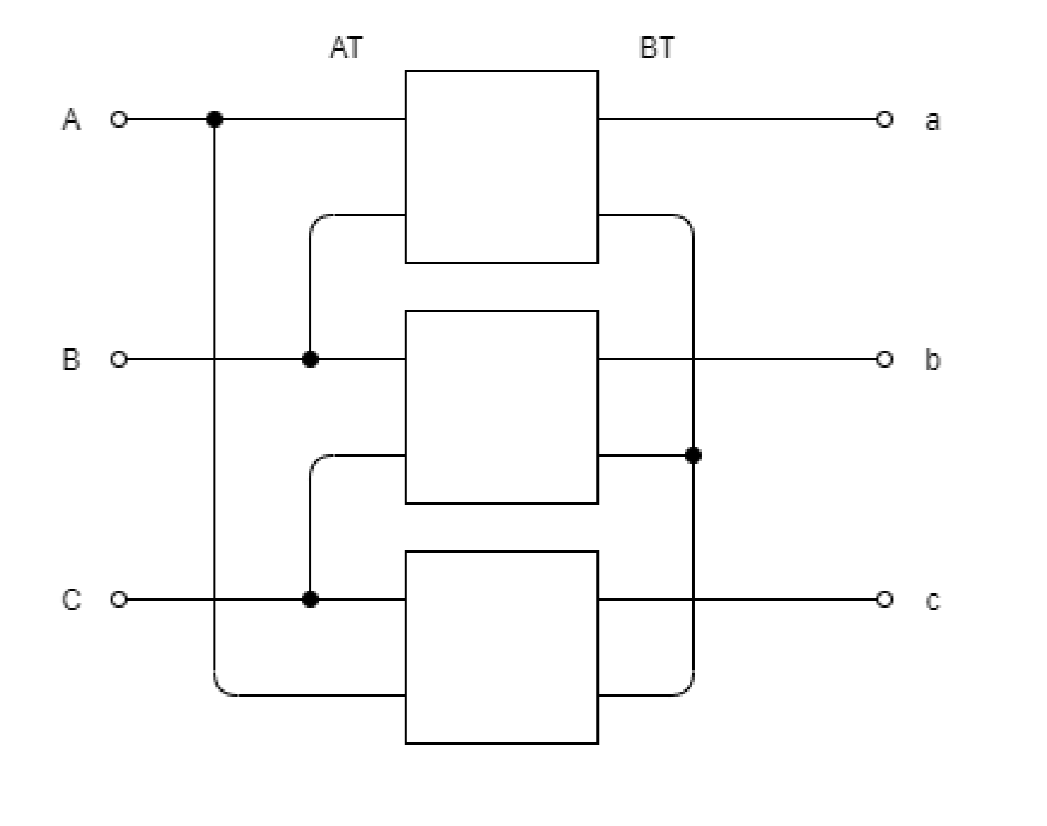
\includegraphics[width=0.5\textwidth]{Jelu_13}
  \caption{Banco trifásico de transformadores: conexiones AT y BT.}
  \label{fig:banco-tri}
\end{figure}

\begin{parts}
  \part Determine el grupo de conexión del banco trifásico usando diagramas fasoriales.
\end{parts}
%---------------------------------------------------------------
\begin{solution}

\subsection*{Resolución 4.a — Grupo de conexión mediante diagrama fasorial}

Dado que \textbf{cada unidad monofásica es de polaridad sustractiva}, las tensiones
fase–neutro de los tres transformadores \emph{están en fase} cuando se observan por separado.

\paragraph{Procedimiento (diagrama fasorial).}
\begin{enumerate}
  \item Dibujar las tensiones \emph{fase–neutro} del lado de \textbf{AT} y fijar
        \(\underline{V}_{AN}\) como referencia (\(0^\circ\)).
  \item Representar las tensiones del \textbf{primario (AT)} considerando su
        \emph{conexión en \(\Delta\)} \(\Rightarrow\) trabajar con fasores \emph{línea–línea}.
  \item Representar las tensiones del \textbf{secundario (BT)} considerando su
        \emph{conexión en \(Y\)} \(\Rightarrow\) fasores \emph{fase–neutro}.
  \item Medir el desfase del conjunto de \textbf{BT} respecto a la referencia de \textbf{AT}.
        En el diagrama se reconoce un desplazamiento
        \begin{equation}
            \angle(\text{BT respecto AT}) = 11 \times 30^\circ = 330^\circ
            \quad(\text{equiv. } -30^\circ).
        \end{equation}
\end{enumerate}

Por lo tanto, el \textbf{grupo de conexión} del banco es
\[
\boxed{\mathrm{Dy11}}
\]
(\(\Delta\) en AT, \(Y\) en BT, con el secundario desfasado \(-30^\circ\) respecto del primario).

\begin{figure}[H]
  \centering
  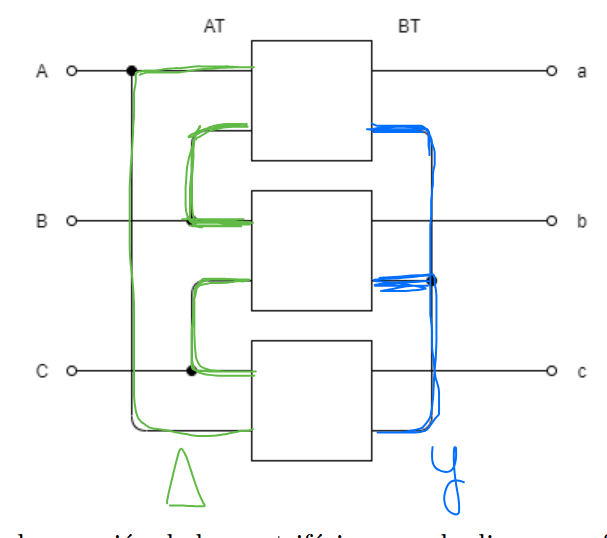
\includegraphics[width=0.6\linewidth]{Jelu_14}
  \caption{Esquema de conexiones de banco de transformadores: lado de alta tensión (AT) en \textbf{Delta} y lado de baja tensión (BT) en \textbf{Estrella} (Y). Las líneas verdes muestran la conexión en triángulo y las azules la conexión en estrella.}
  % alt: Diagrama de tres transformadores con conexiones primarias en Delta y secundarias en Estrella (Y).
\end{figure}
Tenemos que el diagrama fasorial vendra dada por:


\begin{figure}[H]
  \centering
  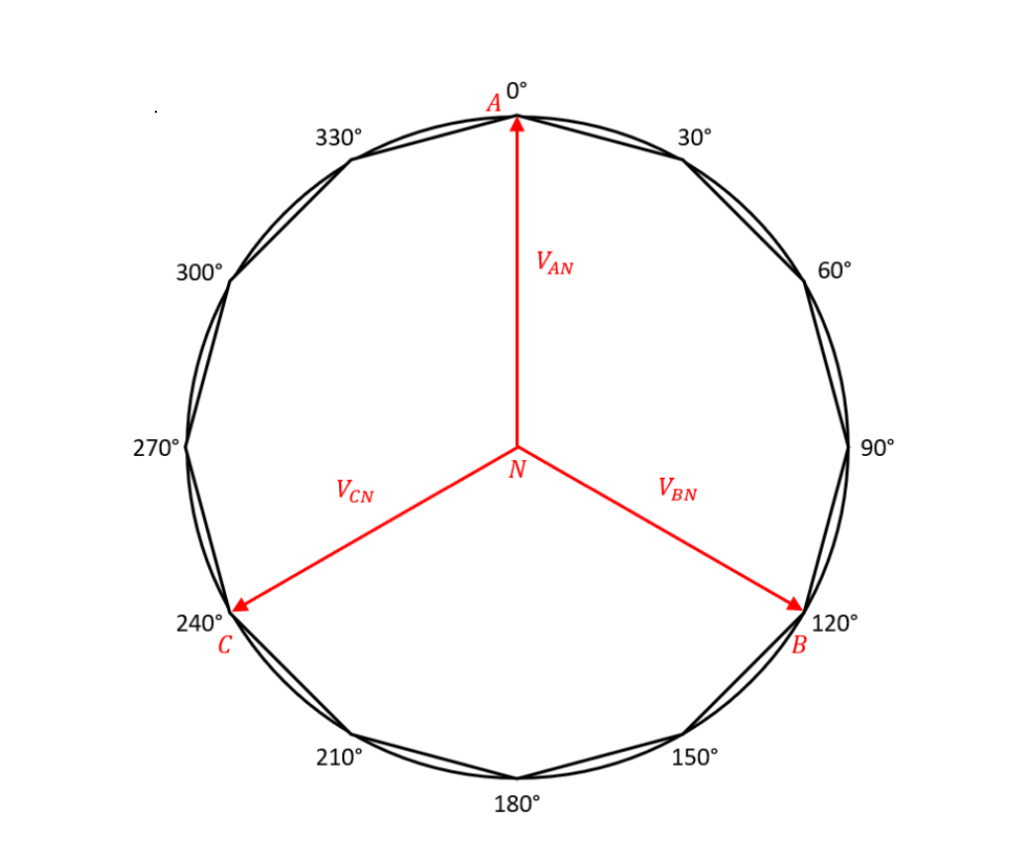
\includegraphics[width=0.6\linewidth]{Jelu_15}
  \caption{Esquema de conexiones de banco de transformadores: lado de alta tensión (AT) en \textbf{Delta} y lado de baja tensión (BT) en \textbf{Estrella} (Y). Las líneas verdes muestran la conexión en triángulo y las azules la conexión en estrella.}
  % alt: Diagrama de tres transformadores con conexiones primarias en Delta y secundarias en Estrella (Y).
\end{figure}


\begin{figure}[H]
  \centering
  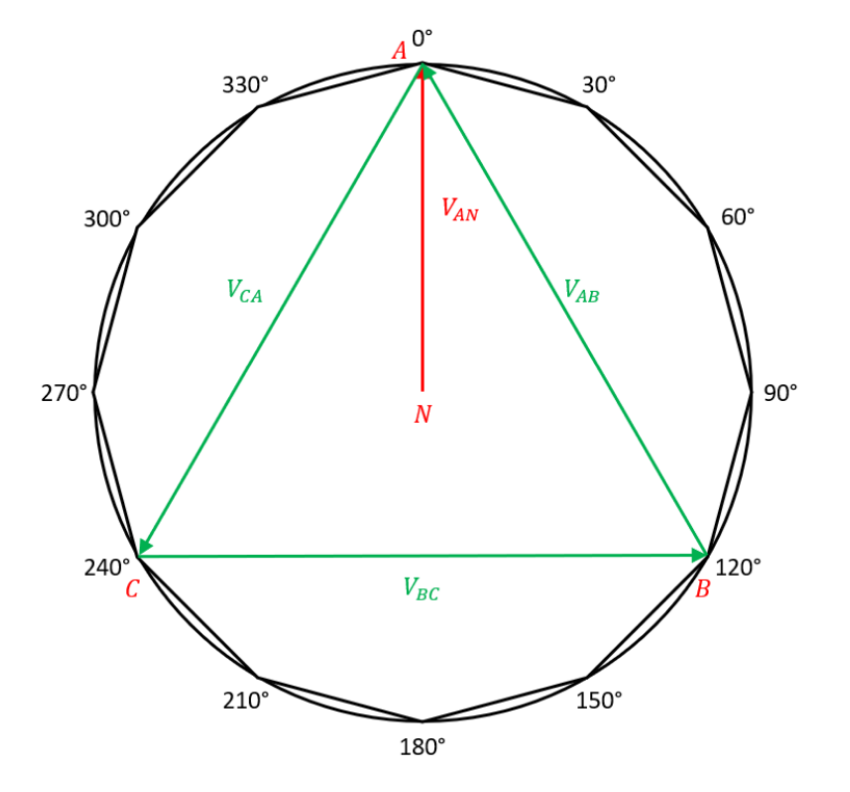
\includegraphics[width=0.6\linewidth]{Jelu_16}
  \caption{Esquema de conexiones de banco de transformadores: lado de alta tensión (AT) en \textbf{Delta} y lado de baja tensión (BT) en \textbf{Estrella} (Y). Las líneas verdes muestran la conexión en triángulo y las azules la conexión en estrella.}
  % alt: Diagrama de tres transformadores con conexiones primarias en Delta y secundarias en Estrella (Y).
\end{figure}

\begin{figure}[H]
  \centering
  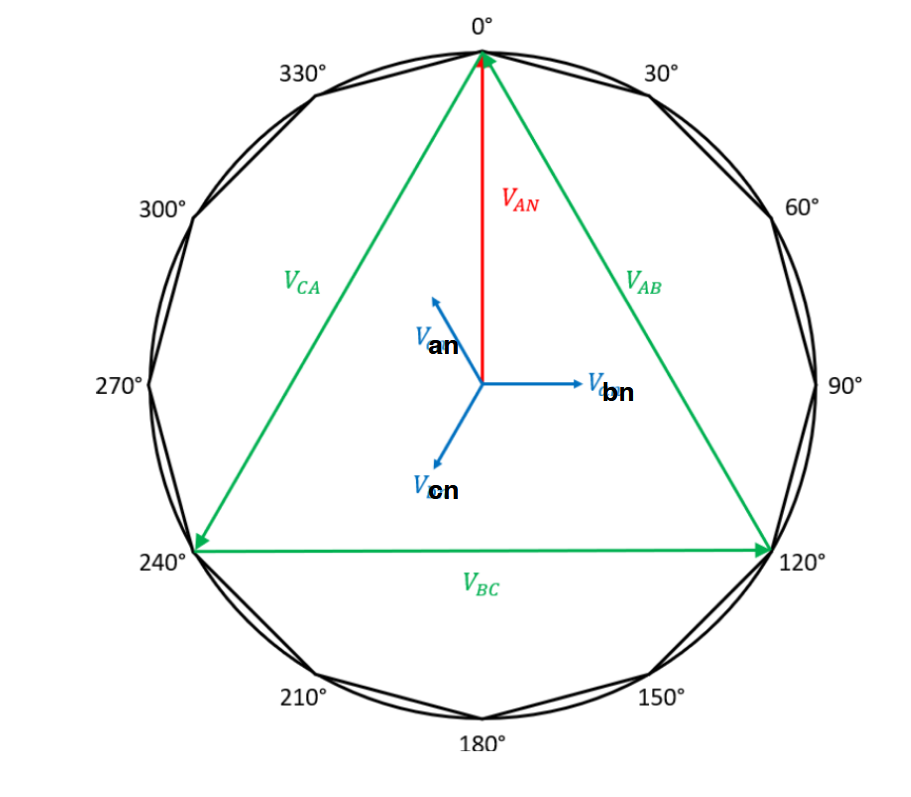
\includegraphics[width=0.6\linewidth]{Jelu_17}
  \caption{Esquema de conexiones de banco de transformadores: lado de alta tensión (AT) en \textbf{Delta} y lado de baja tensión (BT) en \textbf{Estrella} (Y). Las líneas verdes muestran la conexión en triángulo y las azules la conexión en estrella.}
  % alt: Diagrama de tres transformadores con conexiones primarias en Delta y secundarias en Estrella (Y).
\end{figure}
\end{solution}


\end{questions}



\end{document}